\begin{figure*}
    \centering
    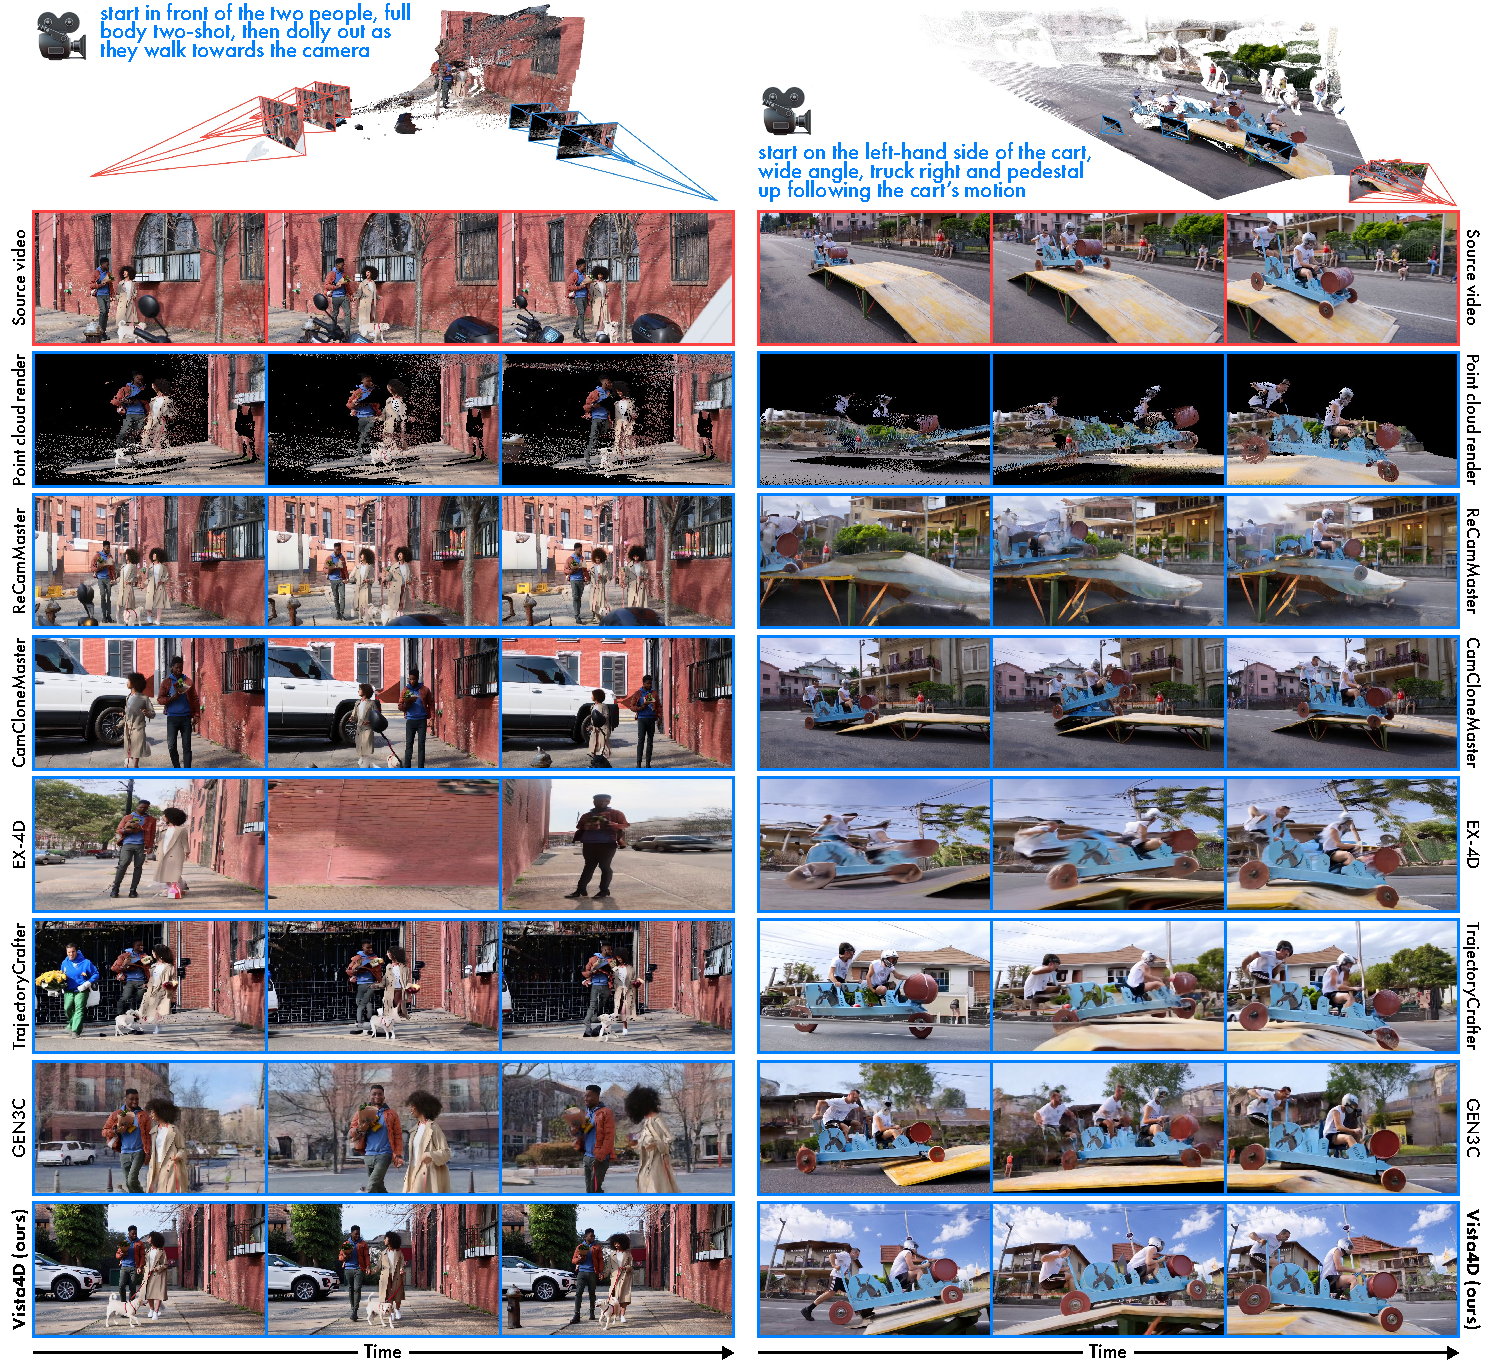
\includegraphics[width=\textwidth]{figures/mid_res/qual_comp.pdf}
    \caption{\Paragraphnoskip{Qualitative comparison on real-life monocular videos} We show two video reshooting examples of \methodname compared to our baselines, TrajectoryCrafter \cite{yu2025trajcraft}, GEN3C \cite{ren2025gen3c}, EX-4D \cite{hu2025ex4d}, ReCamMaster \cite{bai2025recammaster}, and CamCloneMaster \cite{luo2025camclonemaster}.}
    \label{fig:qual_comp}
\end{figure*}

\section{Experiments}
\label{sec:results}

\Paragraph{Baselines} We compare \methodname\ to state-of-the-art video reshooting methods. For explicit-prior methods, TrajectoryCrafter \cite{yu2025trajcraft} introduces the double-reprojection technique to generate training pairs from monocular dynamic videos, EX-4D \cite{hu2025ex4d} proposes the Depth Watertight Mesh during inference to train on tracking-based inpainting, and GEN3C \cite{ren2025gen3c} builds a 3D cache with pooling-based fusion for sparse-view novel-view synthesis. For implicit-prior methods, ReCamMaster \cite{bai2025recammaster} constructs a synthetic multiview time-synchronized video dataset to train a camera-conditioned model, and CamCloneMaster \cite{luo2025camclonemaster} replicates camera trajectories from reference videos. We use our $672 \times 384$ checkpoint for all quantitative evaluations and the user study.

\Paragraph{Evaluation dataset}
For quantitative evaluation, we create an evaluation dataset of high quality, diverse $110$ video-camera pairs: We select $51$ videos from DAVIS \cite{perazzi2016davis} and the royalty-free stock video website Pexels \cite{pexels2025}. Then, we run 4D reconstruction with $\pi^3$ \cite{wang2025pi3} and segmentation with Grounded SAM 2 \cite{ravi2024sam2, ren2024groundingdino, ren2024groundedsam}, and we design two to three camera trajectories for each video with our camera design UI, which we show examples of in Supplementary \ref{supp:eval_user}.

\subsection{Quantitative comparisons}
\label{sec:results:quant}

We quantitatively compare \methodname to baselines and show our method's superiority on three dimensions: Camera control and 3D consistency, novel-view video synthesis, and video fidelity. We include details of each quantitative evaluation metric in Supplementary \ref{supp:quant_metrics}.

\Paragraph{Camera control accuracy and 3D consistency}
We compare camera control accuracy and 3D consistency \methodname to baselines in Table \ref{tab:camera_accuracy} on our $110$ video-camera pair dataset. For camera control accuracy, we measure translation, rotation, and intrinsics error between target cameras from the evaluation dataset and 4D-reconstruction-predicted cameras of generated videos from each method \cite{bai2025recammaster, xu2025virtuallybeing}. For 3D consistency between the source and output videos, following Pippo~\cite{kant2025pippo}, we adopt the per-frame reprojection error of SuperPoint \cite{detone2018superpoint} landmarks under SuperGlue (RE@SG) \cite{sarlin2020superglue}. Our method consistently exhibits more accurate camera control compared to baselines, especially against implicit-prior methods. Moreover, our method significantly outperforms baselines in 3D consistency, showcasing its output geometric plausibility despite noisy real-world 4D reconstruction.

\begin{figure}
    \centering
    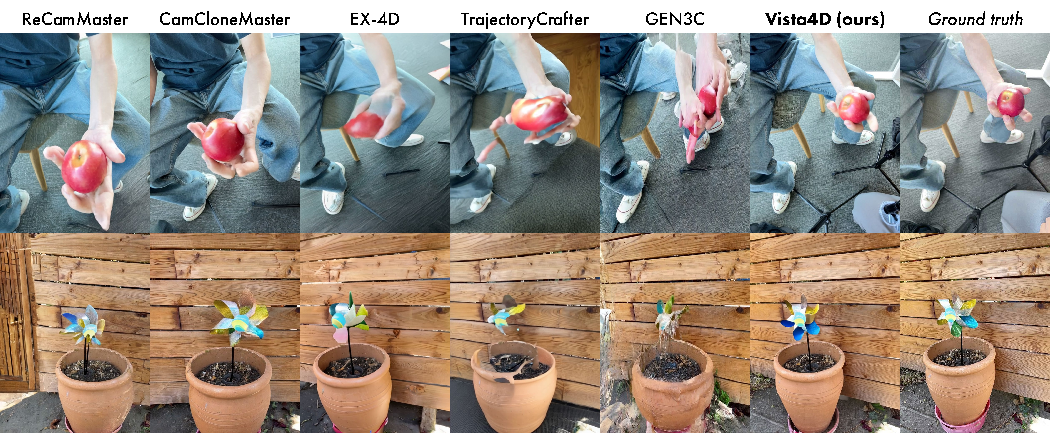
\includegraphics[width=\columnwidth]{figures/mid_res/nvs.pdf}
    \caption{\Paragraphnoskip{Qualitative comparison on novel-view synthesis} We show two samples of \methodname compared our baselines on the \texttt{iphone} dataset \cite{gao2022dycheck}.}
    \label{fig:nvs}
\end{figure}

\Paragraph{Novel-view video synthesis}
We compare novel-view video synthesis quality of \methodname to baselines in Table \ref{tab:nvs} on the real-world time-synchronized multiview dataset, \texttt{iphone} \cite{gao2022dycheck}. We measure masked (indicated by the prefix ``m'') and full PSNR, SSIM, and LPIPS for synthesis quality \cite{gao2022dycheck}, along with optical flow endpoint error (EPE) for motion quality \cite{burgert2025gwtf}. Our method outperforms baselines in PSNR and LPIPS, indicating our superior spatial reconstruction quality. We also significantly outperform baselines for EPE, indicating our method's ability to preserve source video motion. Note that even though we are behind TrajectoryCrafter \cite{yu2025trajcraft} for SSIM, viewing the synthesized videos quickly reveal significant artifacts in the latter's outputs not caught by SSIM, examples of which we show in Figure \ref{fig:nvs}.

\Paragraph{Video fidelity}
We evaluate video fidelity and quality of \methodname to baselines in Table \ref{tab:fidelity} on our $110$ video-camera pair dataset. We use FID \cite{heusel2017fid}, FVD \cite{uterthiner2019fvd}, VBench (aesthetic quality, imaging quality, subject consistency, background consistency, and temporal style) \cite{huang2024vbench}, and VBench-2.0 (human anatomy) \cite{zheng2025vbench2} to evaluate video fidelity, and CLIP-T \cite{radford2021clip} for prompt alignment. Our method consistently outperforms point-cloud-conditioned (explicit-prior) baselines, especially in aesthetic quality, imaging quality, and human anatomy due to our robustness to point cloud artifacts. Implicit-prior methods (ReCamMaster and CamCloneMaster) perform better in FID, FVD, subject consistency, and background consistency because they often fail to follow the target cameras, resulting in relatively little camera change from the source video, which results in seemingly better metrics. Qualitative comparisons in \ref{fig:qual_comp} and Supplementary \ref{supp:qualitative}, along with the user study in Table \ref{tab:user_study}, show our method's clear high video fidelity.

\subsection{Qualitative comparisons}
\label{sec:results:qual}

We qualitatively compare \methodname to baselines in Figure \ref{fig:qual_comp} on two example real-life monocular videos, where we show the point cloud render to illustrate the intended cameras in addition to the written description. Explicit-prior methods (EX-4D, TrajectoryCrafter, and GEN3C) all struggle with point cloud artifacts from target cameras at non-frontal views of the depth maps, resulting in subject and background artifacts (\eg, TrajectoryCrafter, left video; all three methods, right video) or camera control failure (\eg, EX-4D and GEN3C, left video). Implicit-prior methods (ReCamMaster and CamCloneMaster) similarly struggle with precise camera control (ReCamMaster, left video; both methods, right video) and subject artifacts (both methods, left video). In contrast, our method produces high-quality outputs that not only faithfully preserves source video content but also follows the target cameras. We include more comprehensive qualitative results and comparisons in Supplementary \ref{supp:qualitative}.

\Paragraph{User study}
We show the results of our user study in Table \ref{tab:user_study}, where we ask participants to compare our method to baselines on three dimensions: Source video content preservation, camera control accuracy, and overall video fidelity. We randomly select a subset of $30$ video-camera pairs from the $110$-pair evaluation dataset and invite $42$ participants to select their preferred method for each pair and each dimension. Users consistently prefer our method by a wide margin over baselines on all dimensions, especially overall video fidelity due to our method's robustness to point cloud artifacts and challenging camera trajectories and viewpoints. We include details of our user study in Supplementary \ref{supp:eval_user}.

\begin{figure}
    \centering
    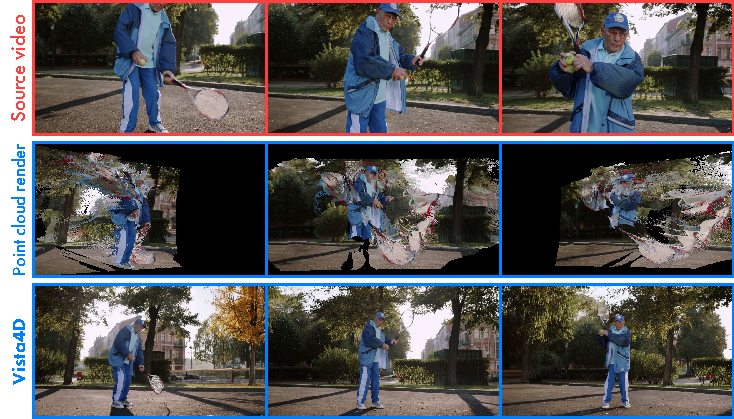
\includegraphics[width=\linewidth]{figures/mid_res/seg_failure.pdf}
    \caption{\Paragraphnoskip{Robustness to segmentation failure} We simulate segmentation failure by not segmenting the tennis racket as dynamic. \methodname is generally robust to these point cloud streaks as it utilizes the in-context-conditioned source video to correct the artifacts.}
    \label{fig:seg_fail}
\end{figure}

\Paragraph{Robustness to segmentation failure}
Since \methodname uses Grounded SAM 2 to segment dynamic pixels, segmentation failures can result in point cloud streaking artifacts. However, \methodname is generally robust to them. For example, we simulate segmentation failure in Figure \ref{fig:seg_fail} by deliberately not segmenting the tennis racket, and \methodname corrects the streaking just like it corrects imperfect point cloud geometry, that is, by utilizing the in-context-conditioned source video. Broadly, we observe that streaking artifacts during inference are rare or inconsequential, especially compared to the improved camera control and 4D consistency from static pixel temporal persistence.

\subsection{Ablation study}
\label{sec:results:ablation}

We study the effects of our data and model conditioning on source video content preservation and robustness to imperfect 4D reconstruction. We perform ablations combinations of the following design choices: No depth artifacts (by always doing double reprojection), no source video, cross-attention source video injection, and no temporal persistence. We find that the combination of training with depth artifacts and the (in-context conditioned) source video enables our model's ability to be robust to 4D reconstruction artifacts, particularly both spatial artifacts (imprecise depths from non-frontal views) and temporal artifacts (jittering depths). We also find that removing temporal persistence reduces our model's ability to both preserve static content and maintain accurate camera control when the source video and target cameras have low per-frame overlap. We show examples of both findings in Supplementary \ref{supp:ablations}.

\begin{figure}
    \centering
    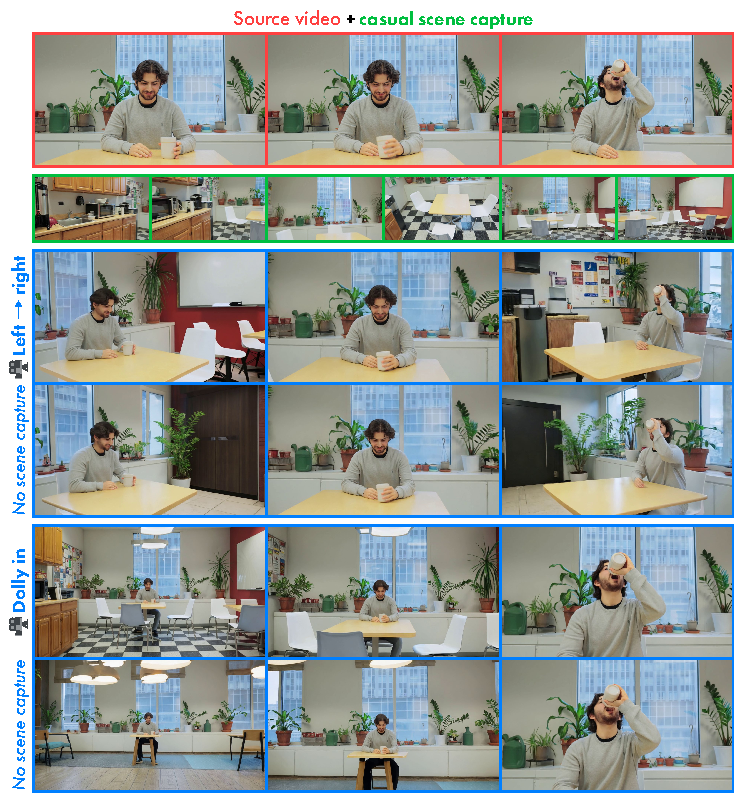
\includegraphics[width=\columnwidth]{figures/mid_res/env_aware.pdf}
    \caption{\Paragraphnoskip{Dynamic scene expansion} With our 4D-grounded temporally-persistent point cloud, \methodname can do video reshooting with additional scene information from casual scene captures or alternate angles by doing joint 4D reconstruction of these frames with the source video. Doing so reduces video model hallucinations and provides stronger control beyond the source video.}
    \label{fig:env_aware}
\end{figure}

\begin{figure}
    \centering
    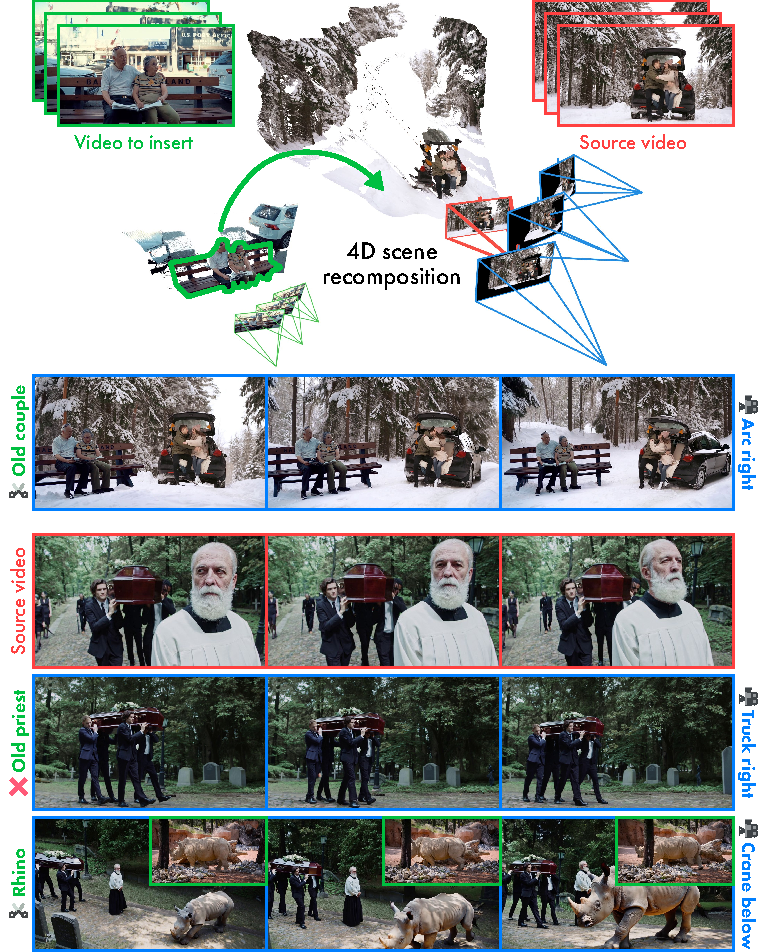
\includegraphics[width=\columnwidth]{figures/mid_res/scene_recomp.pdf}
    \caption{\Paragraphnoskip{4D scene recomposition} By directly editing the 4D point cloud, \methodname can recompose 4D scenes from the source video or other inserted videos. Importantly, our method synthesizes physically plausible lighting when inserting a rhino lit by sunlight through leaves into an otherwise overcast scene.}
    \label{fig:scene_recomp}
\end{figure}

\begin{figure*}
    \centering
    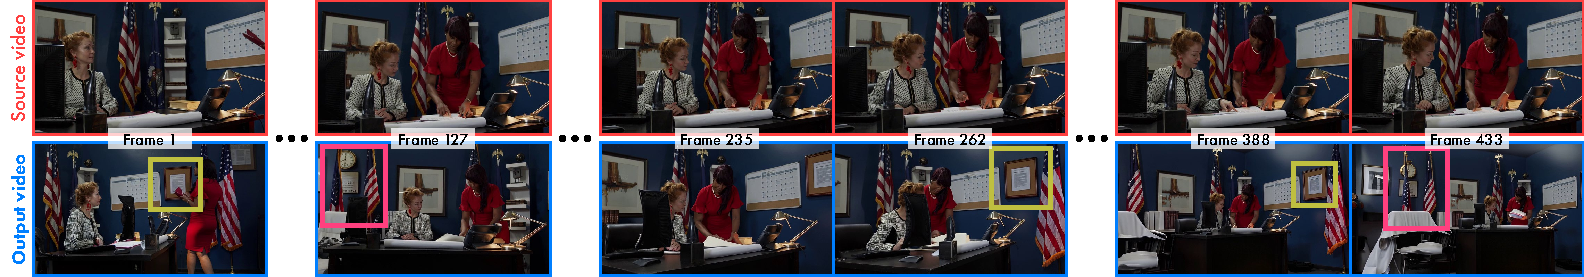
\includegraphics[width=\textwidth]{figures/mid_res/long_video.pdf}
    \caption{\Paragraphnoskip{Long video inference with memory} \methodname can reshoot long videos by doing inference in chunks. By registering static pixels of newly generated chunks back into the temporally-persistent 4D point cloud, \methodname maintains an explicit, 4D-grounded memory of generated content. We showcase this above as the camera arcs around the scene, indicated with color-matched yellow and pink boxes.}
    \label{fig:long_video}
\end{figure*}

\subsection{Applications}
\label{sec:results:app}

\Paragraph{Dynamic scene expansion}
Video reshooting requires the video diffusion models to hallucinate pixels not existent in the source video, even though we often have more visual information of the environment. For example, we may have casual captures of a scene or alternate camera angles on a film set. \methodname's explicit context grounding with temporally-persistent 4D point clouds enables us to incorporate this information by doing joint 4D reconstruction of the source video and additional scene frames. Figure \ref{fig:env_aware} shows an example of dynamic scene expansion, where the addition of temporally-persistent casual scene captures enables more faithful environment reproduction.

\Paragraph{4D scene recomposition}
As \methodname is trained to be robust to point cloud artifacts, we can directly edit and recompose the 4D point cloud to manipulate, duplicate, delete, and even insert new subjects while maintaining their dynamics. Figure \ref{fig:scene_recomp} shows examples of 4D scene recomposition. Notably, the Figure includes an example where we insert the point cloud of a rhino illuminated by sunlight through leaves into an overcast funeral procession scene. Our method naturally blends these differing lighting conditions, generating a region of dappled light around the rhino while keeping the procession in soft shadows under the trees.

\Paragraph{Long-video inference with memory}
For video reshooting on long videos beyond the video diffusion model's trained context window, our temporally-persistent 4D point cloud acts as an explicit, compressed context to retain generated static content across camera viewpoint changes. To do so, we autoregressively generate chunks of the video in target cameras that fit within our model's context window, where we train a variant of our model based on the first-frame-conditioned \texttt{Wan2.1-I2V-14B} to ensure visual consistency between chunks. Figure \ref{fig:long_video} shows an example of long-video inference that retains memory of generated content.
